\documentclass[11pt]{article}
\usepackage{graphicx}
\usepackage{bm}
\usepackage{amssymb}

\setlength{\oddsidemargin}{-0.5cm}
\setlength{\parindent}{1.0cm}
\setlength{\topmargin}{-2.0cm}
\setlength{\textwidth}{16.5cm}
\setlength{\textheight}{25.5cm}

\newcommand{\bc}{\begin{center}}
\newcommand{\ec}{\end{center}}
\newcommand{\ben}{\begin{enumerate}}
\newcommand{\een}{\end{enumerate}}
\newcommand{\bd}{\begin{displaymath}}
\newcommand{\ed}{\end{displaymath}}
\newcommand{\be}{\begin{equation}}
\newcommand{\ee}{\end{equation}}
\newcommand{\bi}{\begin{itemize}}
\newcommand{\ei}{\end{itemize}}
\newcommand{\bt}{\begin{tabbing}}
\newcommand{\et}{\end{tabbing}}
\newcommand{\hs}{\hspace}
\newcommand{\vs}{\vspace}
\newcommand{\lx}{{\LaTeX} }

\newtheorem{exer}{Exercise}

% document body
\title{An Introduction to \lx}
\author{Alison Ramage}
\date{16th March 2017}
\begin{document}
\maketitle

\section{\label{start}Introduction}
\subsection{General Comments}

\lx is a typesetting package widely used by mathematicians. It is
suitable mainly because it makes it easy to produce most
mathematical formulae, cross-referencing for equations and
references is automatic and it is easy to distribute the output
(e.g.\ many journals now prefer \lx manuscripts submitted via the
internet).\\

\lx is based on the more general language, \TeX, which contains a lot of
useful ways of formatting mathematics.
These notes closely follow parts of
\bc
\textit{Learning \lx} (second edition)\\
D.F.\ Griffiths and D.\ J.\ Higham, SIAM 2016
\ec
which is highly recommended as an introductory text.
Other suggested references are
\bc
\textit{\lx: A Document Preparation System}, Leslie Lamport,
Addison-Wesley 1994 (2nd ed.),\\
\textit{The \lx Companion},
F.\ Mittelbach, M. Goossens et al., Addison-Wesley 2004 (2nd ed.),
\ec
both of which contain information about \LaTeXe (which is the
version currently used in most Maths departments). 

\subsection{Running \lx}
As \lx is a typesetting package rather than a word-processor, it
is not an interactive on-screen package. Creating a \lx document
is more like writing a computer program: first you must create a
file containing \lx commands, then `compile' it to process the commands.
The precise method of doing this depends on the type of machine 
that you are using. 

\lx can be run from the command line, that is, by typing commands in a shell 
window (in Linux) or a Command Prompt window (in Microsoft Windows).
Alternatively, it is now fairly common to use a customised \lx User 
`front-end', that is, a
window-based integrated development environment for easy working with \lx (or 
TeX). There are many such environments available: examples of free versions are
\bi
\item \texttt{TeXworks} 
(\texttt{https://tug.org/texworks/}, for Windows and other
operating systems);
\item \texttt{kile} (\texttt{http://kile.sourceforge.net/}, for Mac OS X 
and Linux operating systems);
\item \texttt{overleaf} (\texttt{https://www.overleaf.com/},  
online).
\ei
These notes are based on \texttt{kile}, but \texttt{TeXworks} works in a
similar way.
Both have many options which can be customised to your 
preferences 
once you have some experience. Note that, for this sort of tool, you may need 
to configure the viewing options for PS or PDF files to fit the local 
architecture. \\
\newpage

In general, the steps involved in producing a document in \lx are:
\ben
\item Use an editor to create a file (with extension \textbf{.tex})
containing \lx commands, e.g.\
\textbf{doc.tex}.
\item Compile this, using the \texttt{latex} command or clicking 
on the \textbf{LaTeX} button, to produce a \textbf{
.dvi} (\textit{device independent}) file. Note:
if you are using internal references, you may get the message 
\begin{verbatim}
LaTeX Warning: Label(s) may have changed. Rerun to get
cross-references right.
\end{verbatim}
You must then recompile the file by running LaTeX again.

\item Preview the \textbf{.dvi} file on screen, 
using the \texttt{yap} command or the \textbf{ViewDVI} button,
to check the document layout
(the document will appear in a new window.)

\item Return to step 1: edit the file, re-LaTeX and preview the
changes until you are satisfied that the document is correct.

\item Convert the \textbf{.dvi} file to a format suitable for
printing (i.e., a PostScript file or a PDF file), using the 
\texttt{dvips} command/\textbf{DVItoPS} 
button, or the \textbf{DVItoPDF} button.

\item View the resulting file using an approriate viewer (or by clicking the 
\textbf{ViewPS} or \textbf{ViewPDF} button), and print if required.
\een
\bigskip

\textbf{NOTES:}
\begin{enumerate}
\item It is possible to combine steps 2 to 5 by using the 
\texttt{pdflatex} command (or \textbf{PDFLaTeX} 
button), which LaTeXs your file and produces a PDF file directly which you can 
then view. This can save some time, but does not work with some packages, for 
example, the \texttt{beamer} package described in \S\ref{beamer}.
\item There are several different ways to produce a final PDF file: 
\bi
\item using steps 2-5 above with \textbf{LaTeX} then \textbf{DVItoPDF};
\item using \textbf{PDFLaTeX} as in note 1;
\item using \textbf{LaTeX} and \textbf{DVItoPS} followed by \textbf{PStoPDF}.
\ei
You may have to experiment to see which of theses gives the best end result.
\item
The importance of the previewing stage cannot be
over-emphasised: printing is EXPENSIVE and should only be done when the
document is finalised!
\end{enumerate}

\subsection{\lx errors and warnings}
If your \lx input file contains an error, you will get
an error message (usually with a line number reference) terminated with
a question mark. Most messages are self-explanatory and are
probably the result of typing errors, failure to match brackets or
use of a control sequence (i.e.\ a \lx command) in the wrong
mode. To return to the \$ prompt, type \verb+q+ or \verb+x+. To
interrupt the execution of \lx completely, use Ctrl$\backslash$c or 
Ctrl$\backslash$x.

\lx also frequently generates warnings various potential problems. Mostly, 
these are not crucial but they can be informative. One common message is a 
warning about `overfull and underfull hboxes'. The \textit{overfull 
hbox} warning means that \lx has not been able to find a sensible place to 
place a line break, so the line is slightly too long for the margins. 
Similarly, an \textit{underfull hbox} warning is produced when a line is 
too  short and \lx has had to insert more blank space than it thinks is 
appropriate. You can usually just ignore these but if you are, for example, 
preparing your thesis or a document for journal submission, you may want to 
reword the offending paragraph to solve the problem.
If you use the draft option with the \verb+\documentclass+ command (see 
below) then a black rectangle  will appear in the typeset document wherever an 
overfull hbox occurs, which makes it easier to spot the problem lines.
 


\subsection{Getting started}
\label{starting}
The best way of learning \lx commands is by looking at examples.
The sample file \texttt{wpdoc.tex} and the file used to generate
this document, \texttt{LaTeXnotes.tex}, are both available from the webpage 
\bc
\texttt{https://alisonramage.github.io/latex\_course/}
\ec
You can copy these to your own filespace and
practise running \lx on them. (NOTE: you will also have to copy
the file \texttt{fig1.ps} from the same webpage to produce the figures in
this document). The slides from the accompanying talk (produced in
\lx using the \texttt{beamer} package) are also available as \lx and PDF
files.


\section{Layout of a typical document}

\subsection{ \lx commands}

A \lx source file is a text file which contains the text which you
wish to format and some \lx formatting commands. All \lx commands
begin with a backslash $\backslash$ and are case sensitive. A
command may have a mandatory argument (enclosed in curly brackets)
or an optional argument (enclosed in square brackets).\\

If the text of your document contains any of the following
characters
\bc
\% $\ast$ \$ \& \_ \{ \} \~{} \^{} $\backslash$
\ec
these will be interpreted as \lx control characters. To avoid
this, use

\begin{verbatim}
                   \% $\ast$ \$ \& \_ \{ \} \~{} \^{} $\backslash$
\end{verbatim}
as appropriate.
Note in particular that the percentage sign \verb+%+ acts as a
`comment' symbol in \lx: in your \lx source file, anything on the line 
after a \verb+%+ sign will be ignored.

\subsection{The preamble}

Every \lx document begins with a standard header defining things
like the type of document, the font size, the line spacing etc.
This is known as the \textit{preamble}.\\

The first line of  every \lx document is a 
\verb+\documentclass+
statement which defines the basic format of
the document. It has a mandatory argument denoting the style: the
most common are \verb+article, book, report+ or \verb+letter+. 
These differ mainly in the way the document is broken into sections and how the title page is formatted.
\bi
\item \begin{verbatim}article\end{verbatim}  This is the most commonly-used style: documents of this type
can be divided into sections, subsections and subsubsections, and the 
title is put on the first page along with an abstract and the beginning
 of the text (unless you specify otherwise).
\item \begin{verbatim}report\end{verbatim}  This allows the use of chapters in addition to the above sections,
 although subsubsections are not numbered or indexed. The title is formed 
on a separate page. 
\item \begin{verbatim}book\end{verbatim}  This allows volumes as well as chapters etc. New chapters 
always begin on a right-hand page.
\ei

An example of the command in its simplest form is
\begin{verbatim} 
\documentclass{article}
\end{verbatim} 
However, the \verb+\documentclass+ command also has several optional arguments
which specify typesize, paper size etc., e.g.\ the command
\begin{verbatim} 
\documentclass[12pt,a4]{article}
\end{verbatim} 
will use 12pt text rather than the default 10pt typesize, and use A4 paper for the 
default text region.\\

In theory, this is all that is needed in the preamble. However, it is common
to insert extra commands to define the page size, margins etc. Examples are
\begin{verbatim} 
\setlength{\parindent}{0.0cm}
\setlength{\textheight}{18.0cm}
\setlength{\topmargin}{5.0cm}
\end{verbatim} 
which change the amount by which new paragraphs are indented, the height of
the text region and the size of the top margin respectively. You
may also include any style files or extra packages you may need
with the \verb+\usepackage{+\textit{packagename}\verb+}+ command.\\

The units for specifying distances in \lx can be specified in mm, cm, in
(inches), pt (points), ex or em. A point is a unit used by typesetters
where 72.27pt=1 inch. An ex is the height of a lower case x in the current
font and an em is the height of an upper case M.

\subsection{The document body}

The text to be formatted is immediately preceded by a \verb+\begin{document}+
statement, which must be matched by an \verb+\end{document}+ statement
(which will be the last line in the document). This \begin{verbatim}  
\begin{...}   ...  \end{...} \end{verbatim} 
structure is known as an \textit{environment}, and is an important idea in
\lx: we will see many more examples later.\\

To generate a title, it is easiest to use the \verb+\maketitle+ command:
see wpdoc.tex for an example.\\

The document is structured using paragraphs or sectioning commands. A new
paragraph is started by leaving one or more lines blank in the input document. The
default is for the first line of each paragraph to be indented, and for no
extra vertical space to be inserted between paragraphs. This can be changed 
using  the \verb+\setlength+ command in the preamble with \verb+\parindent+
or \verb+\parskip+. The \verb+\vskip+ command can also be used to leave
extra space between paragraphs: e.g.\ \begin{verbatim}  \vskip 25mm 
\end{verbatim} would leave an extra
25mm between this paragraph and the next. This can be useful if you need
to leave space for a photograph, for example.\\

There are several sectioning commands in \lx including
\bi
\item \verb+\chapter+ (available in book and report styles only)
\item \verb+\section+
\item \verb+\subsection+
\item \verb+\subsubsection+
\ei
These are used by inserting the command with section header in the appropriate
place in the text, e.g.\ the heading for the first section in this document was 
produced by the command 
\begin{verbatim} 
\section{Introduction}
\end{verbatim} 
Note that \lx takes care of all of the section numbering automatically. It
will also create a table of contents using all the chapter, section, subsection
and subsubsection headings if required.

\section{Some useful features}

\subsection{Cross-referencing}
One major advantage of \lx is its ability to automatically number
things like equations and references. Most \lx constructs
(sections, equations, tables, figures etc.) can be given a label using the
\verb+\label{+\textit{labelname}\verb+}+ command which can then be
cited in the text using \verb+\ref{+\textit{labelname}\verb+}+.
 Similarly, references can be cited using the
\verb+\cite{+\textit{bibcode}\verb+}+ command where
\textit{bibcode} refers to the item's label in the bibliography.
See the sample documents for examples of both of these
constructions.

For a larger bibliography, such as that for a PhD thesis, it is a good idea to 
keep your reference list in a separate file and use the \verb+BibTeX+ package 
to keep track of citations. Details of how this is done can be found at
\texttt{http://www.bibtex.org/}.


\subsection{Changing fonts}
A number of fonts are available in \lx. The following \lx segment
\begin{verbatim} 
This text uses the default font, however, \textit{we have now switched to
italics. For some applications} \textsc{small capitals are appropriate, for 
others} \textsl{slanted letters might be useful. To emphasise certain words}
\textbf{bold text can be used. To simulate output from a computer program}
\texttt{the typewriter font is often used and} \textsf{the Sans Serif font has
numerous applications. Now we are} back in the default roman font.

Font changing rules work when the relevant text and command are
enclosed in curly brackets - so we can put \textit{the rest of this sentence into
italics by using curly brackets}. Once the brackets are closed, we revert
to the original font.
\end{verbatim} 
produces the following output:\\

This text uses the default font, however, \textit{we have now switched to
italics. For some applications} \textsc{small capitals are appropriate, for 
others} \textsl{slanted letters might be useful. To emphasise certain words}
\textbf{bold text can be used. To simulate output from a computer program}
\texttt{the typewriter font is often used and} \textsf{the Sans Serif font has
numerous applications. Now we are} back in the default roman font.

Font changing rules work when the relevant text and command are
enclosed in curly brackets - so we can put \textit{the rest of this sentence into
italics by using curly brackets}. Once the brackets are closed, we revert
to the original font.\\

It is also easy to change the size of the text. For example
\begin{verbatim} 
\tiny This text is typeset in ``tiny'' font. \scriptsize is the next largest.
\footnotesize There are several other sizes available \normalsize which allow
you to \large produce a wide range \Large of effects, ranging \LARGE from
tiny labels to \huge large letters suitable for titles and \Huge notices.\\
\end{verbatim} 
produces

\tiny This text is typeset in ``tiny'' font. \scriptsize is the next largest.
\footnotesize There are several other sizes available \normalsize which allow
you to \large produce a wide range \Large of effects, ranging \LARGE from
tiny labels to \huge large letters suitable for titles and \Huge notices.
\normalsize

\subsection{Hyphenation}
\lx is normally fairly good about hyphenating words but will occasionally
find a sentence which it cannot right-justify correctly. It will then
display a warning message concerning an \texttt{overfull $\backslash$hbox}
with the size in points of the error. If the line is only slightly too
long (say less than 20pt) it is unlikely to be noticed. However, you
can specify a ``possible hyphen'' in a word by using $\backslash$-. So
if your document contained the text \verb+long\-word+, \lx would know
that it was permissible to break the line at this point. Alternatively,
the paragraph can be encased in a \verb+\sloppypar+ environment which
causes \lx to relax the rules it uses for formatting paragraphs.

\lx has various rules which tell it where the majority of English words
can be broken, and also contains a list of exceptions to these rules.
If you use specialised words which \lx does not know about, you can add
them temporarily using the \verb+\hyphenation+ command (see manuals).

You may also have a space in your text where you definitely do not want
\lx to insert a new line. In this situation use the tilde $\sim$ 
instead of a space so that the two words will be treated as a single unit,
e.g.\ \texttt{Dr$\sim$Ramage}.

\subsection{Changing the line spacing}
Many documents (in particular theses) are required to be double spaced.
This can be achieved by using the \verb+doublespace+ option in the
documentclass command, i.e.\
\begin{verbatim} 
\documentclass[doublespace]{article}
\end{verbatim} 
Specific parts of the document may be singlespaced using the 
\verb+singlespace+ environment.

Most people find that gaps in a doublespaced document are too large. A
more aesthetically pleasing effect may be obtained by putting a command
such as
\begin{verbatim} 
\renewcommand{\baselinestretch}{1.6}
\end{verbatim}  in the preamble, which increases the line spacing to 1.6 times its normal
value.\\

To force extra space between specific lines, use
\verb+\vspace*{+$x$\verb+cm}+. The equivalent
\verb+\hspace*{+$x$\verb+cm}+ will add extra horizontal space.

\subsection{Footnotes}
Footnotes\footnote{This is an example of a footnote.} are produced using the
\lx command \verb+\footnote{+\textit{text}\verb+}+ at the appropriate point in the 
text\footnote{Footnotes are automatically numbered.}.

\subsection{Processing part of a document}
It is sometimes convenient to split a \lx source file into several
parts, e.g. one file for each chapter of a thesis. This can be done
via the \verb+\include{...}+ command. Parts can then be processed
separately using \verb+includeonly{...}+, as seen in this example:
\begin{verbatim}
\documentclass{book}
\includeonly{chap1,appen1}
\begin{document}
\include{chap1}               % source file chap1.tex for Chapter 1
\include{chap2}               % source file chap2.tex for Chapter 2
\include{chap3}               % source file chap3.tex for Chapter 3
\include{appen1}              % source file appen1.tex for Appendix 1
\include{appen2}              % source file appen2.tex for Appendix 2
\end{document}
\end{verbatim}




\section{Useful environments}
\subsection{Centred text}
Output from \lx is normally left and right justified, i.e.\ the paragraphs
are aligned at both sides. It is sometimes useful to have several lines of
text centred on the page. This is done using the \textbf{center} environment
\begin{verbatim} 
\begin{center}...\end{center}
\end{verbatim} 
Note the American spelling! For example,
\begin{verbatim} 
\begin{center}
This text has been centred. A new line\\
can be forced by adding a double\\
backslash.
\end{center}
\end{verbatim} 
produces
\begin{center}
This text has been centred. A new line\\
can be forced by adding a double\\
backslash.
\end{center}

\subsection{Making lists}
There are three basic types of lists available in \lx - itemised lists,
numbered lists and descriptions. Some examples:

\begin{verbatim} 
\begin{itemize}
\item This is the basic itemised list.
\item Each entry begins with the \verb+\item+ command.
\item Note again the American spelling.
\end{itemize}
\end{verbatim} 
produces
\begin{itemize}
\item This is the basic itemised list.
\item Each entry begins with the \verb+\item+ command.
\item Note again the American spelling.
\end{itemize}

\begin{verbatim} 
\begin{enumerate}
\item Enumerated lists have numeric markers.
\item The numbering is done automatically.
\end{enumerate}
\end{verbatim} 
produces
\begin{enumerate}
\item Enumerated lists have numeric markers.
\item The numbering is done automatically.
\end{enumerate}

\begin{verbatim} 
\begin{description}
\item[The description] environment gives the option of starting each entry
with some bold text.
\item [It is useful] for describing, say, the uses of different commands.
\end{description}
\end{verbatim} 
produces
\begin{description}
\item[The description] environment gives the option of starting each entry
with some bold text.
\item [It is useful] for describing, say, the uses of different commands.
\end{description}

Use of these environments can be quite sophisticated:\\
\begin{itemize}
\item Each of these may be nested.
\item For example
\begin{itemize}
\item this is an itemised list within another list.
\item As you can see the markers have changed automatically.
\end{itemize}
\item and another example \ldots
\begin{enumerate}
\item You can also mix lists.
\item Here is an enumerated lists within an itemised list.
\end{enumerate}
\item Lists can be nested up to four deep, as long as each \verb+\begin+
is matched by an \verb+\end+.
\end{itemize}

\subsection{Tables and boxes}
\subsubsection{The tabular environment}
\lx uses the tabular environment to produces tables, which takes the form
\begin{verbatim} 
\begin{tabular}{column_format}
entry & entry & ... & entry & entry\\
entry & entry & ... & entry & entry\\
\end{tabular}
\end{verbatim} 
where the column format parameters are
\bc
\begin{tabular}{cl}
\textbf{c}& column of centred text\\
\textbf{l}& column of left-justified text\\
\textbf{r}& column of right-justified text\\
\textbf{p\{width\}}& column of specified width\\
\textbf{$|$}& vertical line between columns\\
\end{tabular}
\ec

Divisions between columns are denoted by an ampersand and a double backslash
denotes the end of a line.
For example, the top of the football league table might look like
\bc
\begin{tabular}{lcccccc}
TEAM & PLAYED & WON & DRAWN & LOST & GOALS & POINTS\\
Aberdeen & 2 & 2 & 0 & 0 & +10 & 6\\
Celtic & 2 & 0 & 1 & 1& -5 & 1 \\
Rangers & 2 & 0 & 1 & 1& -5 & 1 \\
\end{tabular}
\ec
which was produced by the \lx commands
\begin{verbatim} 
\begin{center}
\begin{tabular}{lcccccc}
TEAM & PLAYED & WON & DRAWN & LOST & GOALS & POINTS\\
Aberdeen & 2 & 2 & 0 & 0 & +10 & 6\\
Celtic & 2 & 0 & 1 & 1& -5 & 1 \\
Rangers & 2 & 0 & 1 & 1& -5 & 1 \\
\end{tabular}
\end{center}
\end{verbatim} 
Note that the team names are left-justified while the numeric entries are
centred.

\subsubsection{Adding boxes}
You may prefer a boxed table. This can be produced by using the vertical
bar symbol ($|$) in the column-format field and \verb+\hline+ for horizontal
bars. Changing the above input to
\begin{verbatim} 
\begin{center}
\begin{tabular}{||l||c|c|c|c|c|c|}
\hline
TEAM & PLAYED & WON & DRAWN & LOST & GOALS & POINTS\\\hline\hline
Aberdeen & 2 & 2 & 0 & 0 & +10 & 6\\\hline
Celtic & 2 & 0 & 1 & 1& -5 & 1 \\\hline
Rangers & 2 & 0 & 1 & 1& -5 & 1 \\\hline
\end{tabular}
\end{center}
\end{verbatim} 
produces the boxed table
\begin{center}
\begin{tabular}{||l||c|c|c|c|c|c|}
\hline
TEAM & PLAYED & WON & DRAWN & LOST & GOALS & POINTS\\\hline\hline
Aberdeen & 2 & 2 & 0 & 0 & +10 & 6\\\hline
Celtic & 2 & 0 & 1 & 1& -5 & 1 \\\hline
Rangers & 2 & 0 & 1 & 1& -5 & 1 \\\hline
\end{tabular}
\end{center}
\subsubsection{Fixed width columns}
It is also possible to produces a column of a given width. The following
example produces a two-column table with column widths 1.6 and 4.4 inches,
respectively.
\begin{verbatim} 
\begin{tabular}{p{1.6in}p{4.4in}}
\TeX & A typesetting package developed by Donald E.\ Knuth for producing
technical documents. Versions are available for many different computer
systems.\\
\LaTeX & A set of macros for \TeX which make the production of mathematics
based documents much simpler for the average user.
\end{tabular}
\end{verbatim} 
\begin{tabular}{p{1.6in}p{4.4in}}
\TeX & A typesetting package developed by Donald E.\ Knuth for producing
technical documents. Versions are available for many different computer
systems.\\
\LaTeX & A set of macros for \TeX which make the production of mathematics
based documents much simpler for the average user.
\end{tabular}

\subsubsection{One header for several columns}
The \verb+\multicolumn+ option can be used to spread captions over
more than one column. For example:

\begin{verbatim} 
\begin{center}
\begin{tabular}{|c|c|c|c|c|c|}  \hline 
      \multicolumn{6}{|c|}{DTEST.MACRO} \\ \hline
      & Frontal &  \multicolumn{2}{c|}{PCG}
      &  \multicolumn{2}{c|}{EBE} \\ \cline{2-6}
      & CPU & CPU & Its & CPU & Its\\ \hline
      \multicolumn{6}{|c|}{EXP=1} \\ \hline
      125 elements& & & & & \\
      2262 unknowns&54.09&82.68&325 &115.20 &195 \\\hline
      1000 elements& & & & & \\
      4961 unknowns&-&1304.87&674&1304.87&1008 \\\hline
      \multicolumn{6}{|c|}{EXP=5} \\ \hline
      125 elements& & & & & \\
      2262 unknowns&56.21& 99.28 & 396&153.54&262 \\\hline
      1000 elements& & & & & \\
      4961 unknowns&-&1591.35 &822 &1783.12&1241\\\hline
\end{tabular}
\end{center}
\end{verbatim} 
produces

\begin{center}
\begin{tabular}{|c|c|c|c|c|c|}  \hline 
      \multicolumn{6}{|c|}{DTEST.MACRO} \\ \hline
      & Frontal &  \multicolumn{2}{c|}{PCG}
      &  \multicolumn{2}{c|}{EBE} \\ \cline{2-6}
      & CPU & CPU & Its & CPU & Its\\ \hline
      \multicolumn{6}{|c|}{EXP=1} \\ \hline
      125 elements& & & & & \\
      2262 unknowns&54.09&82.68&325 &115.20 &195 \\\hline
      1000 elements& & & & & \\
      4961 unknowns&-&1304.87&674&1304.87&1008 \\\hline
      \multicolumn{6}{|c|}{EXP=5} \\ \hline
      125 elements& & & & & \\
      2262 unknowns&56.21& 99.28 & 396&153.54&262 \\\hline
      1000 elements& & & & & \\
      4961 unknowns&-&1591.35 &822 &1783.12&1241\\\hline
\end{tabular}
\end{center}

\subsubsection{The table environment}
Any of the above tables can be given a caption and label for possible
cross-referencing by enclosing it in the \verb+table+ environment.
The \verb+\begin{table}+ command is followed by an optional argument
specifying the table's position: h for here, t for top of the page or
b for bottom of the page. (\lx may over-ride this however!). An example:
\begin{verbatim}
\begin{table}[h]
\begin{center}
\begin{tabular}{lcccccc}
TEAM & PLAYED & WON & DRAWN & LOST & GOALS & POINTS\\
Aberdeen & 2 & 2 & 0 & 0 & +10 & 6\\
Celtic & 2 & 0 & 1 & 1& -5 & 1 \\
Rangers & 2 & 0 & 1 & 1& -5 & 1 \\
\end{tabular}
\caption{Scottish Premier League Table {\label{prem}}}
\end{center}
\end{table}
\end{verbatim}
produces
\begin{table}[h]
\begin{center}
\begin{tabular}{lcccccc}
TEAM & PLAYED & WON & DRAWN & LOST & GOALS & POINTS\\
Aberdeen & 2 & 2 & 0 & 0 & +10 & 6\\
Celtic & 2 & 0 & 1 & 1& -5 & 1 \\
Rangers & 2 & 0 & 1 & 1& -5 & 1 \\
\end{tabular}
\caption{Scottish Premier League Table {\label{prem}}}
\end{center}
\end{table}

\subsection{Including figures}
\lx provides several different options for handling images from various types 
of file and make them look exactly what you need. In this document, we describe 
one simple approach using the \texttt{graphics} package.
Alternatives are (among many others) the \verb+epsf+ or \verb+psfig+ packages 
which will not be discussed here.

Plots etc.\ in PostScript (.ps) or Encapsulated PostScript (.eps) format can 
easily be included in a document via the \texttt{graphics} package and the 
\verb+\includegraphics+ command. The graphics package must be loaded by 
including the command
\begin{verbatim}
\usepackage{graphicx}
\end{verbatim}
in the preamble. A figure (scaled to the correct size) can then be
produced at the correct point in the text using a \lx segment
similar to the following (which produces Figure \ref{fig1}):
\begin{figure}[!hbtp]
   \begin{center}
     \scalebox{0.5}{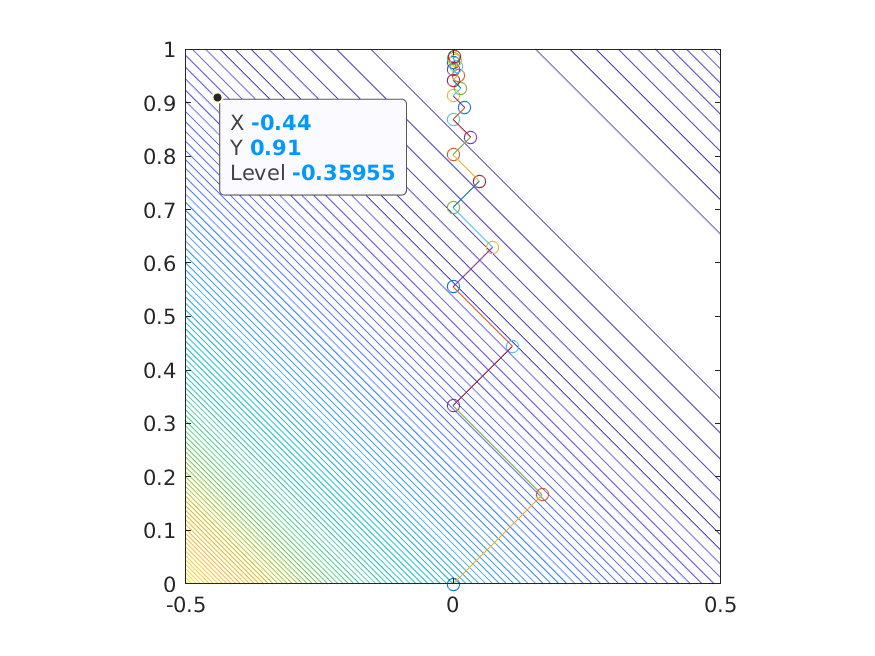
\includegraphics{fig1.png}}
   \end{center}
   \caption{An example of including a picture.\label{fig1}}
\end{figure}
\begin{verbatim}
\begin{figure}[!hbtp]
   \begin{center}
     \scalebox{0.5}{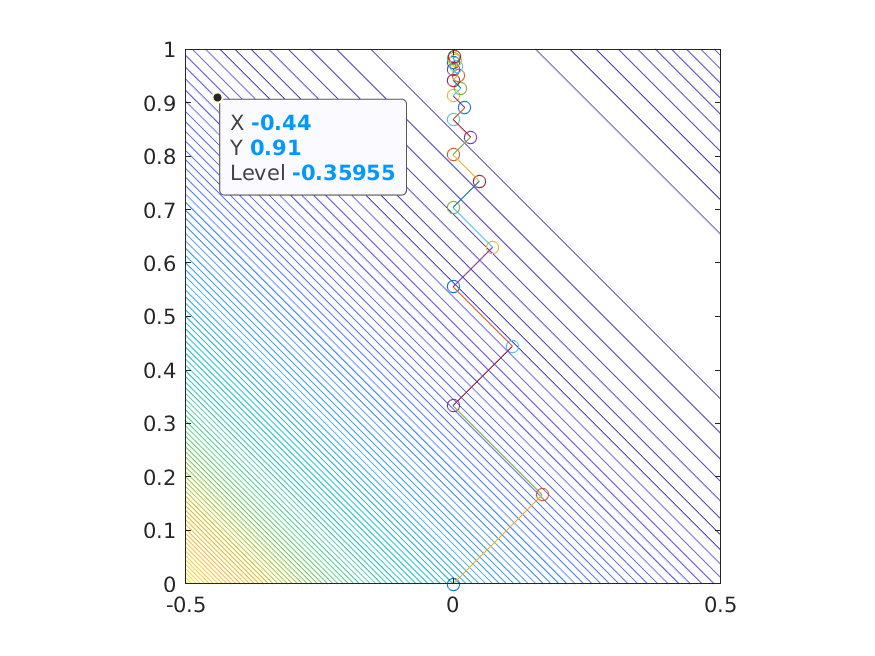
\includegraphics{fig1.png}}
   \end{center}
   \caption{An example of including a picture.\label{fig1}}
\end{figure}
\end{verbatim}
The \verb+figure+ environment allows the inclusion of captioned
pictures and diagrams and is used in a very similar way to the \verb+table+
environment discussed above. The optional argument again specifies the figure's 
preferred position in order of preference: h for here, t for top of the page or 
b for bottom of the page (the inclusion of ! with these options means that 
this really is your preferred position, even if \lx would automatically 
override this).
The numerical argument of \verb+\scalebox+ can be changed to alter the size of 
the
picture.\\

More complicated spacing of graphs can be managed by using the minipage
environment. For example, Figure \ref{fig2} is created by the \lx segment
\begin{verbatim}
\begin{figure}[hb]
\begin{center}
\mbox{
   \begin{minipage}{2.5in}
   \scalebox{0.3}{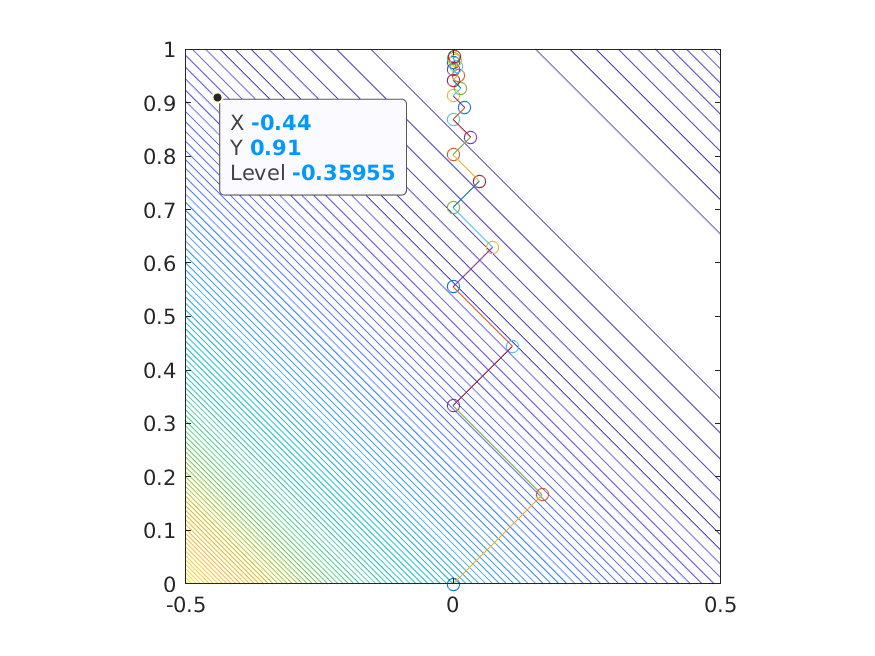
\includegraphics{fig1.png}}\\
   {\small (a) Picture 1.}\end{minipage}\qquad
   \begin{minipage}{2.5in}
   \scalebox{0.3}{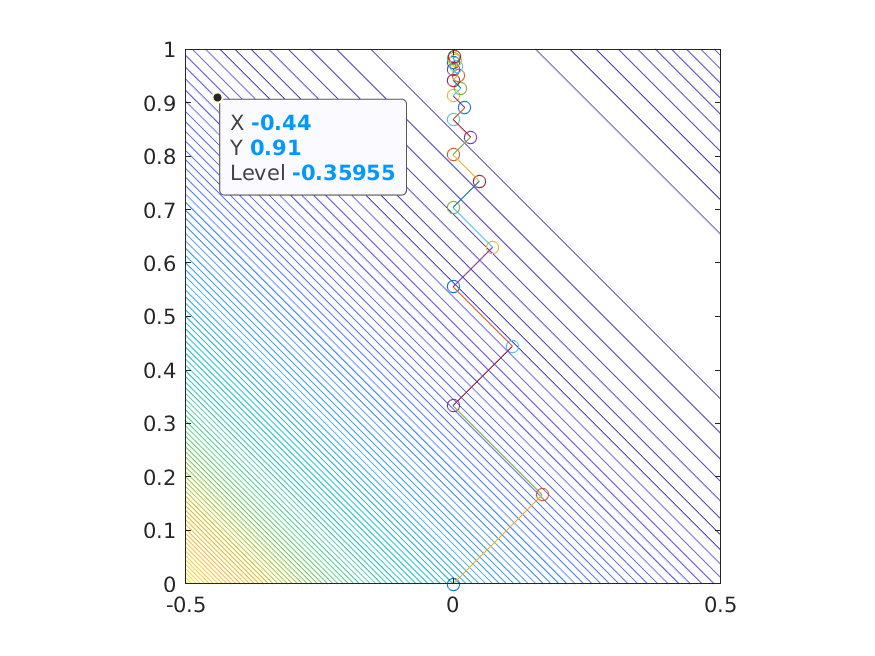
\includegraphics{fig1.png}}\\
   {\small (b) Picture 2.}\end{minipage}
}\\
\end{center}
\begin{center}
\mbox{
   \begin{minipage}{2.5in}
   \scalebox{0.3}{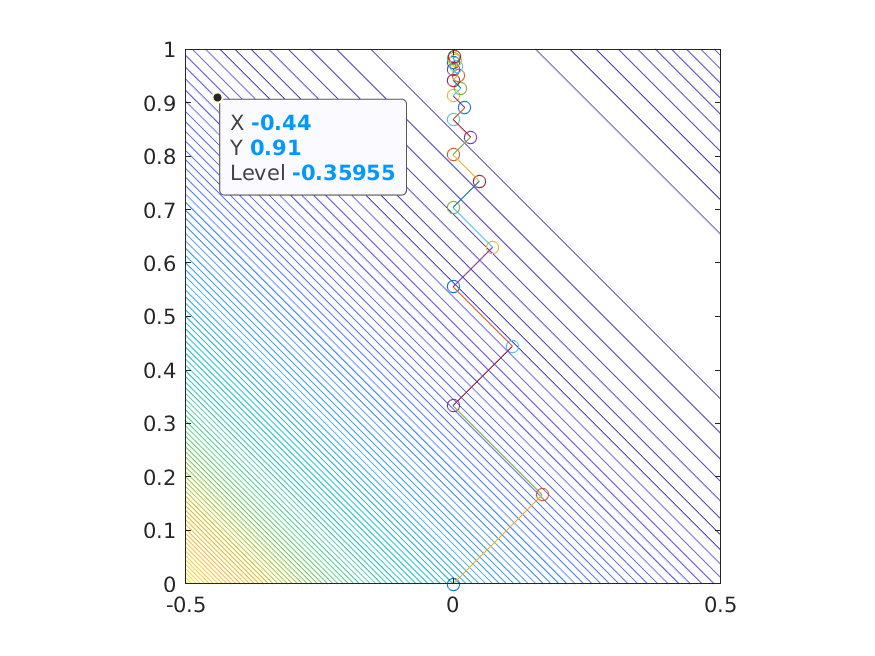
\includegraphics{fig1.png}}\\
   {\small (c) Picture 3.}\end{minipage}\qquad
   \begin{minipage}{2.5in}
   \scalebox{0.3}{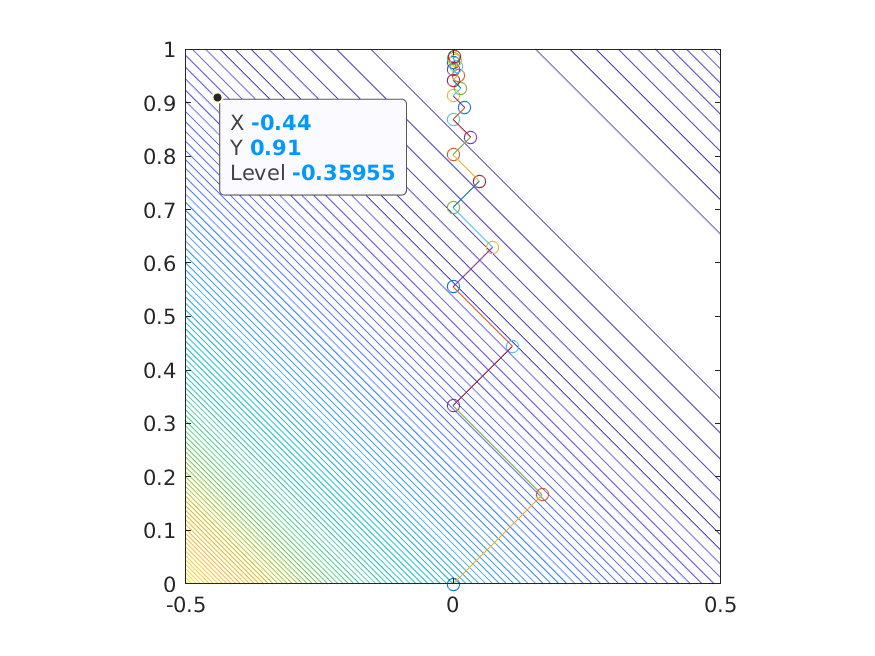
\includegraphics{fig1.png}}\\
   {\small (d) Picture 4.}\end{minipage}
}\\
\end{center}
\caption{An example  displaying more than one picture.\label{fig2}}
\end{figure}
\end{verbatim}
\begin{figure}[hb]
\begin{center}
 \mbox{
 \begin{minipage}{2.5in}
 \scalebox{0.4}{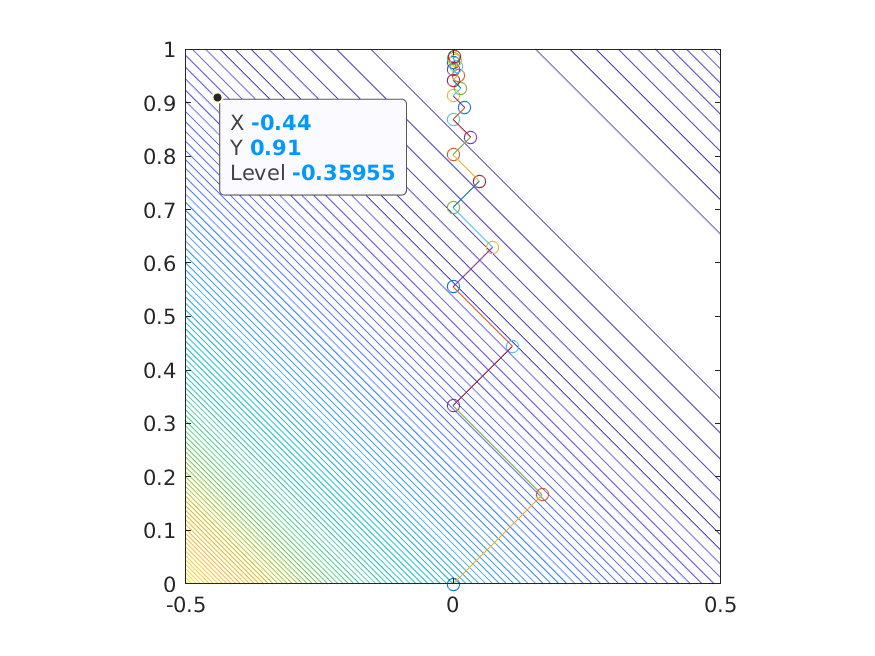
\includegraphics{fig1.png}}\\
 {\small (a) Picture 1.}\end{minipage}\qquad
 \begin{minipage}{2.5in}
 \scalebox{0.4}{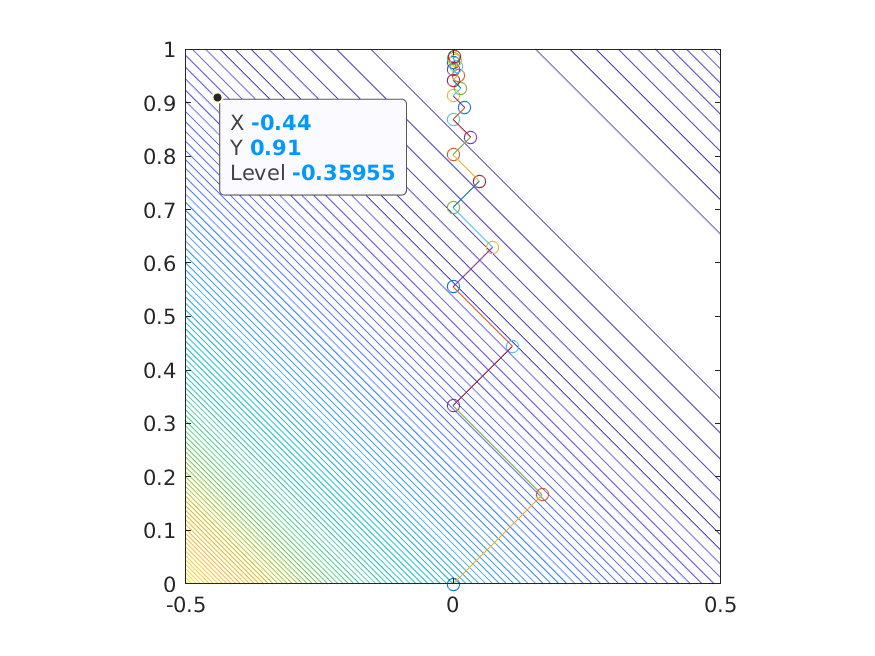
\includegraphics{fig1.png}}\\
 {\small (b) Picture 2.}\end{minipage}}\\
\end{center}
\begin{center}
 \mbox{
 \begin{minipage}{2.5in}
 \scalebox{0.4}{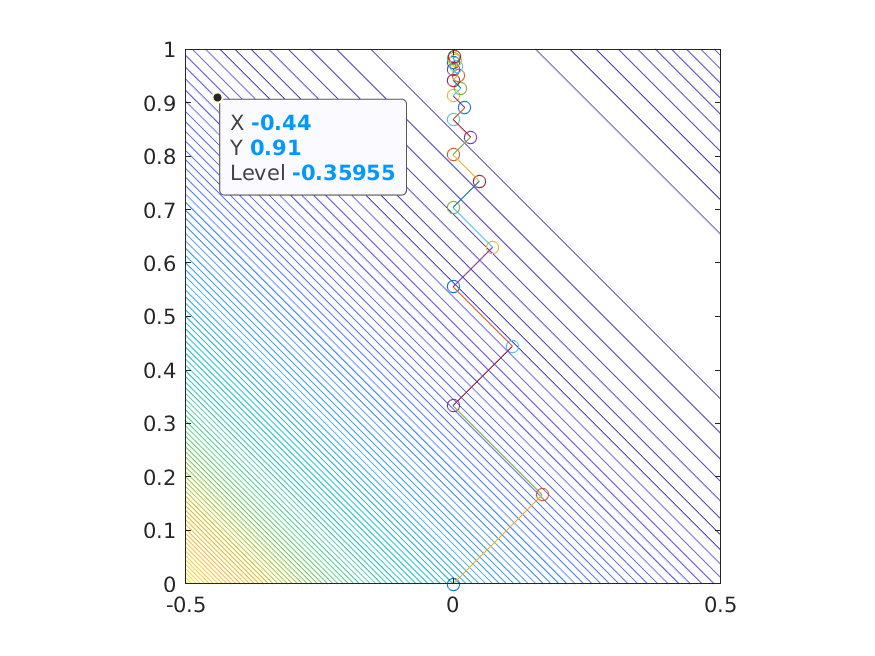
\includegraphics{fig1.png}}\\
 {\small (c) Picture 3.}\end{minipage}\qquad
 \begin{minipage}{2.5in}
 \scalebox{0.4}{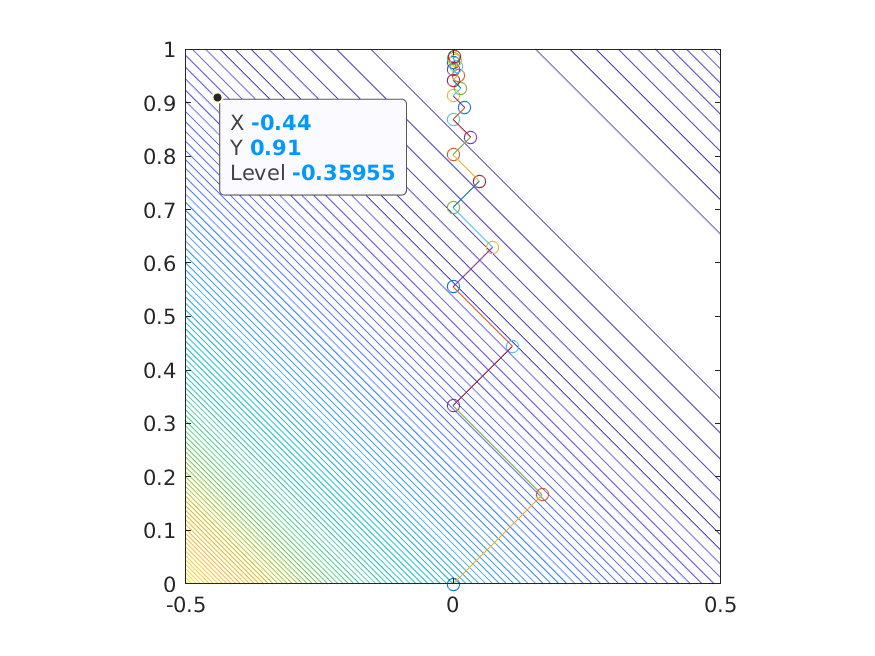
\includegraphics{fig1.png}}\\
 {\small (d) Picture 4.}\end{minipage}}\\
\end{center}
 \caption{An example  displaying more than one picture.\label{fig2}}
\end{figure}

\subsection{Verbatim}
The \verb+verbatim+ environment is useful for printing things like
computer code or raw \lx as it prints out the text exactly as it was
input in typewriter font. This has been used a lot in preparing this 
document.



\section{Mathematical Formulae}

Only a few examples of the mathematical capabilities of \lx can be
given here: for detailed information, consult the books listed in
section~\ref{start} and the sample file wpdoc.tex or search online. 

\subsection{Math mode}
Mathematics in \lx must be typeset in math mode. There are two basic 
forms: \textit{inlinemode} and \textit{displaymode}. Inline mode is
indicated by enclosing the \lx command between two \$ signs. For
example,
\begin{verbatim}
This line contains $E=mc^2$, $A=2\pi r$ or $x=\frac{1}{2}y$.
\end{verbatim}
produces\\

This line contains $E=mc^2$, $A=2\pi r$ or $x=\frac{1}{2}y$.\\

There are many ways of using displaymode. The most usual is the
\textit{displaymath} environment, which centres the formula on the
page in its own space, e.g.\
\begin{verbatim}
\begin{displaymath}
v_{i}=\sin{\frac{i\pi}{N+1}}.\\
\end{displaymath}
\end{verbatim}
gives\\
\begin{displaymath}
v_{i}=\sin{\frac{i\pi}{N+1}}.\\
\end{displaymath}
The same effect is obtained by enclosing the expression in double
dollar signs \verb+$$...$$+.\\

If you wish to number an equation for reference purposes, use
instead the \verb+equation+ environment:
\begin{verbatim}
\begin{equation}
\label{psieq}
\psi_{i}=\frac{1}{6i}-\ln{\frac{1}{2}}.\\
\end{equation}
\end{verbatim}
which gives\\
\begin{equation}
\label{psieq}
\psi_{i}=\frac{1}{6i}-\ln{\frac{1}{2}}.\\
\end{equation}

\noindent The \verb+\label+ statement means that you may refer to the
equation in the text using \verb+\ref{psieq}+.

To format several lines of equations, use the \verb+eqnarray+
environment. As in the \verb+tabular+ environment, equations are
lined up using ampersands. For example,

\begin{eqnarray}
\epsilon\nabla^2\psi & = & -\rho \\
q\frac{\partial p}{\partial t} & = & -\nabla.J_p-qR \nonumber \\
q\frac{\partial n}{\partial t} & = & -\nabla.J_n-qR 
\end{eqnarray}

was produced by

\begin{verbatim}
\begin{eqnarray}
\epsilon\nabla^2\psi & = & -\rho \\
q\frac{\partial p}{\partial t} & = & -\nabla.J_p-qR \nonumber \\
q\frac{\partial n}{\partial t} & = & -\nabla.J_n-qR 
\end{eqnarray}
\end{verbatim}

Note the use of \verb+\nonumber+ in the second line. If you wish 
none of the equations to have numbers, use the \verb+eqnarray*+
environment instead.

\subsection{Building formulae}

The strategy for building mathematical formulae is quite
straightforward: simply start at the left and work along
``translating'' each term and remembering to match all brackets.
Some common expressions:
\bc
subscripts - \verb+$expr1_{expr2}$+ produces $expr1_{expr2}$\\
superscripts - \verb+$expr1^{expr2}$+ produces $expr1^{expr2}$\\
fractions - \verb+$\frac{expr1}{expr2}$+ produces $\frac{expr1}{expr2}$\\
square root - \verb+$\sqrt{expr1}$+ produces $\sqrt{expr1}$\\
sum - \verb+$\sum_{k=1}^n a_k$+ produces $\sum_{k=1}^n a_k$\\
integral - \verb+$\int_{x=0}^\infty e^{-x^2}dx$+ produces $\int_{x=0}^\infty e^{-x^2}dx$\\
limit - \verb+$\lim_{n\to\infty}(1-\frac{x}{n})^n$+ produces
$\lim_{n\to\infty}(1-\frac{x}{n})^n$\\
derivative - \verb+$\frac{\partial f}{\partial x}$+ produces
$\frac{\partial f}{\partial x}$
\ec

Horizontal space in equations can be added using \verb+\quad+
and \verb+\qquad+: smaller spaces come from e.g.\ \verb+\,+ (thin space),
\verb+\:+ (medium space), \verb+\;+ (thick space) or \verb+\!+ (negative thin 
space).

Hats, tildes and other `maths accents' may also be easily obtained. For
example,
\begin{verbatim}
\begin{displaymath}
\hat{x},\,\tilde{v},\:\dot{u},\;\ddot{u},\quad\underline{f+g},\qquad\overline{a+b}.
\end{displaymath}
\end{verbatim}
produces
\begin{displaymath}
\hat{x},\,\tilde{v},\:\dot{u},\;\ddot{u},\quad\underline{f+g},\qquad\overline{a+b}.
\end{displaymath}

You can typeset your formulae in different fonts using the commands
\begin{center}
\verb+\mathbf+, \verb+\mathit+, \verb+\mathsf+, \verb+\mathcal+
\end{center}
to obtain bold, italic, sans serif and calligraphic fonts, respectively (used in
the same way as for normal text). To produce bold versions of Greek letters, 
one option is to use the \verb+\bm+ command from the \texttt{bm} package.
Note that spaces are ignored in math mode: to
put some normal text into a maths expression, use the \verb+\mbox+ command. For
example, use
\begin{verbatim}
\begin{displaymath}
x^2-1>0\mbox{ for all }x>1.
\end{displaymath}
\end{verbatim}
to produce
\begin{displaymath}
x^2-1>0\mbox{ for all }x>1.
\end{displaymath}

\subsection{Brackets}
In addition to square and round brackets, we may use curly brackets in 
equations provided they are proceeded by a backslash \verb+\{...\}+.
To get brackets adjusted in size to fit a particular formula, use
\begin{verbatim}
\left\{ \left[ \left( \left| ... \right| \right) \right] \right\}
\end{verbatim}
noting that each \verb+\left+ MUST be accompanied by a \verb+\right+, even
if the bracket type is not the same (use \verb+\left.+ or \verb+\right.+ if
you don't want any bracket printed).

\subsection{Arrays}
The \verb+array+ environment is used for formatting arrays or matrices,
and it must be used in mathmode. It is similar to the \verb+tabular+
environment: the position of the entries within each column is specified by
c, l or r, entries are separated by ampersands and lines are ended by a double
backslash. For example, the \lx segment
\begin{verbatim}
\begin{displaymath}
A=\left[\begin{array}{ccc}
1 & 1 & 1\\
x & y & z\\
x^2 & y^2 & z^2
\end{array}\right], \quad
x=\left[\begin{array}{r}
1 \\ -2 \\ 4
\end{array}\right]
\end{displaymath}
\end{verbatim}

produces
\begin{displaymath}
A=\left[\begin{array}{ccc}
1 & 1 & 1\\
x & y & z\\
x^2 & y^2 & z^2
\end{array}\right], \quad
x=\left[\begin{array}{r}
1 \\ -2 \\ 4
\end{array}\right]
\end{displaymath}

Ellipsis of various kinds may also be useful here. For example,
\begin{verbatim}
\begin{displaymath}
T=\left[\begin{array}{ccccc}
a & b & 0 & \cdots & 0\\
c & a & b & &\vdots\\
0 &\ddots&\ddots&\ddots& 0\\
\vdots & &c & a & b \\
0&\cdots &0&c & a
\end{array}\right]
\end{displaymath}
\end{verbatim}
produces
\begin{displaymath}
T=\left[\begin{array}{ccccc}
a & b & 0 & \cdots & 0\\
c & a & b & &\vdots\\
0 &\ddots&\ddots&\ddots& 0\\
\vdots & &c & a & b \\
0&\cdots &0&c & a
\end{array}\right]
\end{displaymath}


\section{Abbreviations}
Typing common \lx commands over and over can be tedious. New \lx commands
which are shorter can be defined using \verb+\newcommand+. For example,
if the abbreviations
\begin{verbatim}
\newcommand{\beq}{\begin{equation}}
\newcommand{\eeq}{\end{equation}}
\end{verbatim}
are defined in the preamble, then \lx will expand every occurrence of
\verb+\beq+ in the text to \verb+\begin{equation}+. See the text of this
document for more examples.

\section{Packages and style files}
The basic \lx commands can be greatly enhanced by using packages and style files. 
For example, many publishers provide style files (which can be downloaded from 
their website) to be used by contributing authors to set up articles in the 
journal's preferred style. The American Mathematical Society packages 
\texttt{amsmath}, \texttt{amsfonts} and \texttt{amssymb} can be particularly 
useful for producing special mathematics characters like $\mathbb{R}$, 
$\mathbb{N}$, $\mathbb{Z}$ etc.
Several common packages are already 
distributed with 
\texttt{MiKTeX} and \texttt{kile}. Many other packages and style files are 
accessible via the UK\TeX archive \texttt{http://www.tex.ac.uk}. These can 
also be customised to produce personalised style files.

You can include a package or style file in your \lx document using the 
\verb+\usepackage+
command in the preamble. For example, 
\begin{center}
\verb+\usepackage{exam}+
\end{center}
will include the style file \textbf{exam.sty}. 


\section{Slides and presentations}
\label{beamer}
There is more than one way to prepare slides in \LaTeX. One popular style 
to use is 
\bc
\verb+\documentclass{beamer}+,
\ec
 which is very similar to the \verb+article+ style except that the 
\texttt{frame} environment
\begin{center}
\verb+\begin{frame} ... \end{frame}+
\end{center}
is used to produces a series of separate slides. The slide style, colour etc.\ 
can be specified using the \verb+\theme+ and \verb+\colortheme+ commands. 
There are many sources of further information about \verb+beamer+ available 
online. In particular, The \lx file used to produce the slides which accompany 
these notes, \texttt{LaTeXslides.tex}, is available on the course webpage 
(see \S\ref{starting}). Note that slides produced with \texttt{beamer} cannot 
usually be viewed in DVI format: you should first convert to PS or PDF format 
to view your draft slides.

\section{Posters}
One method of producing a large poster to display your research results is by 
using the \texttt{a0poster} document class
\bc
\verb+\documentclass[a0]{a0poster}+
\ec
(although other classes can be used). This will produce an A0 paper sized 
poster in landscape format. Other than offering additional font sizes, such as
\bc
\verb+\veryHuge+,
\verb+\VeryHuge+, and
\verb+\VERYHuge+,
\ec
this is very like the \verb+article+ document class.

\end{document}
